\documentclass[10pt,notitlepage]{article}
\usepackage[a4paper, top=0.6in, left=0.6in, right=0.6in, bottom=0.6in]{geometry}
\usepackage[utf8]{inputenc}
\usepackage[english]{babel}
\usepackage{hyperref}
\usepackage{csquotes}
\usepackage[style=ieee]{biblatex}
\usepackage{amsmath}
\usepackage{amssymb}
\usepackage{graphicx}
\usepackage{caption}
\usepackage{subcaption}

\graphicspath{{images/}}
\addbibresource{references.bib}

\title{
  {Real or Not: How Does the Use of Natural Language Processing Improve the Classification of Disaster Tweets?}\\
  {\large Machine Learning, Group 97. Vrije Universiteit Amsterdam}
}
\author{
  Hongyu He
  \and Beata Haracewiat
  \and Matthias Debernardini
  \and Alexander Balgavy
  \and Soufiane Jounaid
}
\date{\today}

\begin{document}
  \maketitle

  \begin{abstract}
    Twitter is home to 321 million active users from all over the world.
    It is 36th on Alexa, and the verb ``tweet'' is now a mainstay in the English vernacular.
    Today, when news breaks, it breaks first on twitter.
    Often, when a disaster emerges, tweets begin to flood the Twittersphere about the situation.
    For emergency dispatchers, becoming aware of an accident as it unfolds and proactively deploying resources to the location can have a profound impact on the collateral damage.
    However, this necessitates the need for an intelligent system that can process and interpret tweets because no person or group of people can read and understand the constant stream of tweets.
    Because these tweets are mainly composed of natural language, the intelligent system needs to process the natural language so that it can output actionable suggestions.
  \end{abstract}

  \section{Introduction}
In this report, we describe the NLP (Natural Language Processing) pipeline to compete in the ``Real or Not? NLP with Disaster Tweets'' Kaggle competition.
The goal of the competition is to decide, given a tweet, whether it pertains to a disaster or not.
The NLP pipeline with the highest accuracy wins the competition.
The prepared dataset was provided by Figure Eight Inc.
and the pipeline consisted of Python libraries.

\subsection{Hypothesis}
Our research will focus on exploring the difference in the models’ performance depending on the feature set. Similar research has shown the potential
of NLP feature extraction techniques to improve the predictions \cite{y1,y2,y3}.
Thus, our research will focus on investigating the hypothesis: \textit{Linguistic features extracted using the natural language processing pipeline
improve the classification of disaster tweets compared to classic derivable features.}

\subsection{Approach}
In order to investigate our hypothesis, we have decided on a structured approach.
As the first step, we performed pre-processing on the provided training data, which included data analysis and data cleaning.
This step consisted of investigating the class imbalance, dealing with missing values and seeking correlations between features and classes among others.
Based on the latter we have built a set of features which could be potentially useful for the classification.
These will be later used for the training pipeline.
For model evaluation, cross-validation with 5 stratified folds was used.
This ensured that every instance from the dataset has been used for the training at least once.
Moreover, the folds contained approximately the same proportion of the target value as the original dataset.
To form the final conclusions, we evaluated our models on the test data.
The respective steps along with the reasoning are described in-depth in the following sections.


  \section{Method}
\subsection{Data preprocessing}

The dataset required some initial preprocessing.
\autoref{tab:columns-null-counts} below shows the columns present in the training dataset, along with the amount of instances that did not have a value for the given column.
The keyword is a word associated with (or representative of) a given instance, the location is optionally entered by the user when they are authoring a tweet, the text is the content of the tweet, and the target is the label of the tweet.

\begin{table}[h!]
  \centering
  \vspace{1em}
  \renewcommand{\arraystretch}{1.5}
  \begin{tabular}{| l | c |}
    \hline
    \textbf{Column} & \textbf{Amount of instances with a null value for the column} \\ \hline
    keyword & 61 \\ \hline
    location & 2533 \\ \hline
    text & 0 \\ \hline
    target & 0 \\ \hline
  \end{tabular}
  \renewcommand{\arraystretch}{1}
  \vspace{1em}
  \caption{}
  \label{tab:columns-null-counts}
\end{table}


The first observation we made was that out of the total 7613 instances, none of them were missing a target label.
This meant that all of the data was usable for supervised training and validation.
Furthermore, all instances have an entry for the text column, so this column would be useful for feature extraction.

We then saw that 61 instances were missing a value for the keyword column, which is approximately 0.8\% of the whole dataset.
Out of those 61 instances, 42 were labelled as positive and 19 as negative. Based on this, we decided to fill in the missing data by imputation: for the positive instances, we filled in the mode of the keyword for positive instances, and likewise for the negative instances. We reasoned that this was fine, as it would not really affect the dataset as a whole, since only a small percentage of the dataset had a missing value for that column. Furthermore, there was no significant difference between the amount of positive versus negative instances that had a missing value for `keyword'.

In the case of the location, around one third of the instances had a null value for this column.
Unfortunately, in this case it was not possible to do much: using the mode value for the location would not make sense, and we did not have enough other features which we could use to train a model to predict the location of an instance (predicting this from just the text would be difficult). Moreover, missing data for the location could also be expected in the real-world use case. Therefore, we decided to leave the empty values empty, and potentially create a model that could use the location values when present.

Next, we had to deal with duplicate instances in the dataset.
There were no strict duplicates (i.e. duplicates where every column was duplicated); however, there were 69 instances that contained repeated text values. Out of those 69 rows, 37 rows contained the same text, yet were labelled differently. As this would be confusing for our model during training, we decided to simply drop rows with duplicated labels, because we did not have a good method to keep only the rows that were labelled correctly (doing this manually could lead to errors caused by subjectivity). Dropping duplicate rows did not have a major impact on the size of the dataset, as the operation only removed 110 instances, or around 1.44\% of the data.

Some cleaning of the text values was also necessary, as they contained HTML entities and abbreviations that would not be understood by our natural language processing (NLP) pipeline, but could still carry meaning.
In particular, we replaced HTML entities (e.g. \verb|&amp;|) with their English-word equivalent (e.g. ``and''). We also expanded abbreviations to their full form, e.g. ``ER'' to ``emergency room''.

Finally, we noted the class imbalance of the dataset, which is shown in \autoref{tab:class-imbalance}:

\begin{table}[h!]
  \centering
  \vspace{1em}
  \renewcommand{\arraystretch}{1.5}
  \begin{tabular}{| l | l | p{0.4\linewidth} |}
    \hline
    \textbf{Class} & \textbf{Number of instances} & \textbf{As percentage of total number of instances} \\ \hline
    1 (is a disaster) & 3198 & 42.62\% \\ \hline
    0 (is not a disaster) & 4305 & 57.38\% \\ \hline
  \end{tabular}
  \renewcommand{\arraystretch}{1}
  \vspace{1em}
  \caption{}
  \label{tab:class-imbalance}
\end{table}

There were approximately 14.76\% more negative instances than there were positive instances.
The class imbalance problem arises when one class is represented by significantly more instances than the other class \cite{Japkowicz2002}.
In our case, we decided that this distribution was tolerable and would not lead to a major problem, given the size of the data.

\subsection{Extracting features from the text}

Some of the columns, such as the keyword, would be immediately usable as a feature.
However, the text still required further processing.

Some of the text values contained character sequences that had special meanings when used on Twitter.
For example, alphanumeric strings beginning with an ``@'' symbol are ``mentions'', and are used to directly refer to another user's Twitter account in a message.
Alphanumeric strings beginning with a ``\#'' symbol are ``hashtags'', and are used to categorise a message (a user may add one or more categories which they deem fitting for their message).
In our processing, we decided to also treat these two kinds of alphanumeric strings accordingly, as their presence could be a useful feature.

Overall, we noted the presence of several kinds of entities in the text: mentions of relief organisations, mentions of news organisations, other mentions, hashtags, organisations (companies, agencies, institutions, etc.), geopolitical entities (countries, cities, states), and facility entities (buildings, airports, highways, bridges, etc.).
For each mention present in a message, we also noted whether the mentioned user was a known news organisation (e.g.
CNN, BBC) , or a known relief organisation (e.g.
MSF, Oxfam), as this could be a good indicator of whether the message referred to a disaster.


We checked whether the hashtags in a message and the message itself contained a synonym of the word ``disaster'' or ``accident''; we obtained these synonyms from Roget's 21st Century Thesaurus.
These synonyms were split up into `levels': level 1 synonyms were synonyms deemed closer in meaning to the word `disaster', and level 2 were less similar.
We also extracted the subject, verbs, and objects for each sentence in each message, as these three grammatical features are generally part of the
independent clause, and are useful in determining the topic of a sentence or message \cite{nordquist}.
Finally, we checked whether the text contains words that could be used to describe ‘damage’, such as `explode' or `rupture'.

\subsection{Feature selection}
After processing the data, some analysis was necessary to determine which features would be useful in a model.
To begin, we computed for each potential feature the amount of messages that had a value for that feature; you can see the results in
\autoref{tab:feature-stats} in the appendix.

Some of the features we extracted do not occur very frequently in the dataset.
For example, only 0.03\% of the tweets in the dataset have a hashtag that is a level 2 synonym of `disaster', which amounts to two tweets.
The same is true for level 1 synonyms of `disaster', which occur in 0.12\% of the hashtags of the tweets (9 instances).
This means that they may not be useful features to consider, as they do not occur very often in general.

Similarly, mentions of news organisations and relief organisations do not occur very often either: they are contained in 0.95\% (71 instances) and 0.04\% (3 instances), respectively.
One reason for this may be that the list of Twitter accounts that we are using is too limited, and the tweets in our dataset simply refer to other news or relief organisation accounts.
Unfortunately, there is no straightforward way of compiling a fully complete list of such accounts.
Moreover, these features may still be useful, as if they are present, they may immediately be a strong indicator of the labelling of the message; to determine whether this is the case, further analysis was necessary, as discussed below.

When selecting features for inclusion in the model, we created plots and attempted to find potential correlations.
Firstly, we looked at only the columns that were already provided in the dataset.
For the keywords, we observed that generally, a keyword is not equally as often associated with positively labelled tweets as it is with negatively labelled tweets.
This is shown in \autoref{fig:keywords-vs-target} in the appendix, which is an excerpt from the full plot: the turquoise section (representing the amount of positive instances) and the red section (representing the amount of negative instances) are rarely the same size.
The full plot is not included here for brevity; nevertheless, this excerpt should serve to show that the keyword can be a good indicator of the label.
There are some discrepancies that are worth mentioning, namely that different forms of the same word (e.g.
noun, adjective, adverb, plural, singular) may indicate different class labels.
For example, the keyword `deaths' generally indicates that an instance should be labelled as positive, whereas for keywords `death' and `dead', it is more likely that the instance is negative.
This is probably because the English language contains many words whose meanings change depending on the context, or whether they are meant figuratively.

The location column was not useful, for two reasons.
Firstly, it is entered by the user, so it either may be spelled in an unusual way (e.g.
``M!\$\$!\$\$!PP!" meaning ``Mississippi''), or even be a valid location.
This is not trivial to clean or analyze, and due to time constraints, we did not investigate ways to do so.
Secondly, there is no location present for one-third of the training dataset.
Therefore, we decided not to consider this in our models.

Although, as shown above, less than one percent of the dataset contained a direct mention of a news organisation's account, it could still be used as a feature.
As can be seen in \autoref{fig:mentioned-news} in the appendix, if a message mentions a news organisation, it is more likely that it should be labelled as positive.
Therefore, if present, we could potentially use this feature to predict a positive label for the instance.

Next, we analyzed the presence of level 1 synonyms of `disaster'.
As is shown in \autoref{fig:contains-l1} in the appendix, the difference is not that significant, but it is still somewhat more likely for the tweet to be labelled as positive when it contains a synonym than when it does not.
Similar plots were created for level 2 synonyms and words relating to damage; these plots are omitted for brevity, but the results show that these two features would not be a good indicator of the instance being positive.

We also observed that tweets labelled as positive have a higher number of recognised entities (geopolitical entities, organisations, and facilities) in the text.
This can be seen in \autoref{fig:num-ents-vs-target} in the appendix, where if a tweet contains five or more entities, it becomes more likely that it is a positive instance.
However, there are only a handful of tweets with seven or eight entities, so it is possible that this observed `relationship' may actually be a result of the small size of the training dataset.

Finally, we investigated the role of hashtags in the classification of tweets.
As we said above, not many hashtags contained synonyms of the word `disaster'.
However, for those that did, it is clear from \autoref{fig:hashtags-contain-synonyms} in the appendix that they were mostly labelled as positive.


We also considered the number of hashtags present in a tweet, and observed that as the number of hashtags increases, it is generally more likely that the tweet should be labelled as positive.
However, this is not a clear relationship, as there are some outliers.
\autoref{fig:num-hashtags-vs-target} and \autoref{fig:num-hashtags-vs-target-zoomed} in the appendix show the same plot, but \autoref{fig:num-hashtags-vs-target-zoomed} was zoomed in by plotting only tweets with four or more hashtags to make potential relationships more visible.
These figures show that there is a higher proportion of positively labelled tweets that contain seven or more hashtags, but there are some outliers, such as at nine and eleven hashtags.
Furthermore, similarly to the number of entities, it is important to consider that this apparent relationship may actually result from the small size of the training dataset.
Nevertheless, the number of hashtags could still be a useful feature for label prediction.

Another reason for the hashtags in a tweet to potentially be a useful feature is that the most popular hashtags for the labels differ significantly.
As can be seen in \autoref{fig:top-30-hashtags-false} and \autoref{fig:top-30-hashtags-true} in the appendix, out of the 30 most commonly occurring hashtags in each class, only four are the same for positive (turquoise) and negative (red) instances.
In addition, those four hashtags are relatively generic: ``best'', ``hot'', ``news'', and ``prebreak''.
This means that if a specific hashtag occurs in a given text, it is a likely indicator of the label that should be predicted for that instance.


  \section{Experiments}
In an effort to carry out a proper experiment, we applied a variety of methods to our data.
From Natural language processing to non-linear models, the following subsection describes the motivation behind the choices we made in this department and outlines our performance predictions.

We experimented with two techniques for our baseline models, excluding our linguistic features of course, because one of the primary questions we aim to answer in this paper is whether the added linguistic features we extracted using the natural language processing pipeline improve the classification of disaster tweets compared to classic derivable features.

\subsection{First attempt: Logistic regression}

For our first baseline model, we wanted a simple and statistical approach.
Logistic regression serves our purpose nicely, taking multiple numerical features and outputting a binary response probability.
In this specific case we employ this model with 2 feature extraction methods: Bag of words and Term frequency-inverse document frequency (TF-IDF).
Bag of words is a simple text feature extraction method, it builds a vocabulary of unique words it encounters throughout the input and keeps a measure of their occurrences.
TF-IDF takes the concept a step further by multiplying the measure (term frequency) by the term's inverse document frequency: in our setting this translates to multiplying the frequency of a word in a tweet by a measure of how rare or common it is in the corpus (set) of tweets.

Term frequency Inverse document frequency in our setting is defined as:

$$
\text{TFIDF} = \frac{\text{number of occurrences of a term}}{\text{total number of words in the tweet}} \log{\Big( \frac{\text{total number of tweets}}{\text{number of tweets containing the term}} \Big)}
$$

The logistic regression model then uses a logit function to estimate probabilities. This function is defined as:

$$
F(x) = \frac{1}{1-e^{-x}}
$$

where

$$x = w_0 + \sum_{k=1}{n} w_k \cdot x_{k}$$

$w_k$ are the regression coefficients of the model and $x_k$ are the features.
The results of this model can be depicted in a confusion matrix, as shown in \autoref{fig:confusion-matrix} in the appendix.
These results are particularly bad, considering we have a large amount of false positives, meaning that a large number of non disaster related tweets were classified as disaster, if we consider cost imbalance, this is not as bad as having the opposite scenario.
We can conclude on this basis that this regression model is indeed a bit brave (classifies most data points as positive).

\subsection{Experimental setup: The Pipeline}

To enable several experiments using different classification methods, some sort of pipeline needs to be established.
To turn our data set in training data points, we assemble together a 5 component pipeline.

The Data preprocessing elaborated in previous sections is the first part of our pipeline,this section handles data cleaning and exploration, i.e generating more features.
Consequently, the training data points become more and more complex throughout the pipeline, both in terms of data type and format.
At the end of the process, the training data contains numerical, textual and categorical labeled data.
Therefore, the second part of the pipeline is a column transformer from the Scikit-learn library which is responsible for serializing all kinds of extracted features from every column into scalar values.
Then, the third part of the pipeline is a scalar which normalises these scalar values to the same range in order to prevent bias.

The experimental part is the fourth part, which is regarded as a slot where different classification methods are “plugged in” to produce predictions.
Finally, the last part of the pipeline is the evaluation of the predictions, for this matter we used cross-validation with 5 stratified folds for all experiments, furthermore the loss measurement is based on the mean square error (MSE) of the classifiers.
We rely on this measure as a primary means to compare classifiers and test our hypothesis
In an effort to carry out a proper experiment, we applied a variety of methods to our data.
From Natural language processing to non-linear models, the following subsection describes the motivation behind the choices we made in this department.and outlines our performance predictions.

We experimented with two techniques for our baseline models excluding our linguistic features to help us answer the research question.

\subsection{Baseline method: Linear SVC with derivable features (non-NLP)}
The method that we used for our baseline is Support Vector Classifier (SVC), a statistical model built using support vector machines.
The goal behind SVM is to find the decision surface that maximizes the margin between the data points of the two classes (disaster related or not in this case).
This decision surface is best illustrated through the following figure from \cite{4}:

\begin{figure}[h]
  \centering
  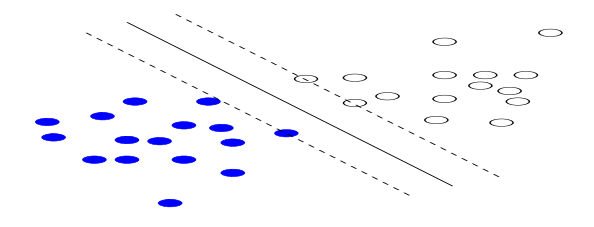
\includegraphics[scale=0.5]{decision-surface.png}
  \caption{A decision line (solid) and a margin (distance between dashed lines), both represent the decision surface.}
  \label{fig:decision-surface}
\end{figure}

Mathematically, this decision surface (for linearly separable data) can be written as a hyperplane \cite{4} where the vector x is a data point we want to classify whereas w and b are learned from the training set :

$$vec(w_i) \cdot vec(x_i) - b = 0$$

Let $y_i$ be the classification of a data point $vec(x_i)$. If it evaluates to +1 for positive and -1 for negative, the SVM optimization problem can be simply written as the following two inequalities:

$$
\begin{cases}
  vec(w_i) \cdot vec(x_i) - b \geq +1, &\text{for } y_i = +1 \\
  vec(w_i) \cdot vec(x_i) -b \leq -1, &\text{for } y_i = -1
\end{cases}
$$


One way to motivate this choice for our task would be to showcase comparative studies involving SVM and text classification, and indeed we do provide a few studies showing that Support Vector Machines can provide state-of-the-art performance in text classification tasks \cite{3,4}.
We will show later that our Linear variant of SVC however loses horsepower against its non linear counterparts, this is partly due to our added NLP features breaking the linear separability property of our dataset.
More on this in the next section.

\subsubsection{Feature Pre-elimination}

Before deploying the linear SVC method, we were eager to evaluate the usefulness of some features.
To this end, we set up a quick comparison (not using our full pipeline) comparing the results of using the id feature or not.
As expected, The metrics shown in table \autoref{fig:feature-pre-elim-metrics} demonstrate that the id feature has a negative impact on the prediction, we decided to omit it for later stages.

\subsubsection{Exploiting Feature Space with Kernel Tricks}

Before we proceed with adding more and more features, we need to uncover some properties of the training data.
In this subsection we employ a variety of kernels for our SVC model (using kernel trick), furthermore based on the results we will be able to make assumptions about the shape and condition of the data.


First, an assumption is made that the feature space before extracting more features should be linearly separable.
To prove this, several experiments using SVC with 3 kernel types, rbf \cite{x1}, polynomial and sigmoid, are conducted.
It turns out, based on the results shown in table \autoref{fig:rbf-kernel-tricks} and \autoref{fig:poly-kernel-tricks}, this is indeed the case that the linear kernel outperforms other 2 non-linear kernels using only basic features serialized from the original dataset.
Our assumption holds so far.
Furthermore, based on the training set accuracy, the SVC with \verb|poly| kernel seems to have overfitted and the overall standard deviation of the predictions is quite high.

\subsection{Non-baseline methods: (NLP) Entity-related Features}

Without using any NLP-related features, the performance of the prediction is about 50 - 60\% accuracy if taking the variations into account. The current scores are by no means close to yielding a useful model. However, since the feature space is still rather naïve, exploring more features with natural language processing seems promising.

To build our NLP component, we used one of the best performing NLP libraries at the moment, SpaCy \cite{x2,x3}. Since concrete entities are  reflected through the tweets, we will use these as central features and derive the other features from them. Following this protocol, we end up with 5 features : the entities themselves,  the labels/types of the entities, the words dependent on the entities (Part of speech), the positions of the entities in a sentence (Part of speech) and the derived words of the entities.

\subsubsection{SVC - The Second Try}
Having the previous performances on hand, more experiments were undertaken using SVC.
Similar to the previous method, an experiment using the linear kernel was first conducted.
Then, experiments using non-linear kernels are followed.
The results of experiments in question are summarised in \autoref{fig:linear-kernel-svc}, \autoref{fig:rbf-kernel-svc},
\autoref{fig:poly-kernel-svc}, and \autoref{fig:sigmoid-kernel-svc} in the appendix.


As a corollary, the performances of most of the non-linear kernels have surpassed that of the linear kernel.
We, therefore, conclude that, after adding the 5 entity-related features, the feature space is no longer linearly separable.
Most importantly, the scores of the predictions have been improved a lot which gives away the possibility of having further improvement by adding more relevant features.
In addition, the prediction produced by the polynomial kernel is exceptionally bad, therefore we decided to omit it from the next experiment.

\subsubsection{Classification ensemble with Adaboost}

Although the performance got improved by adding those entity features, the bias of the results remains huge as the accuracy is still below 65\%.
Thus, ensemble methods with boosting \cite{x4} in turn become the next attempt with the purpose of reducing bias and improving accuracy.
An adaboost classifier is then plugged into the pipeline.
The results of this experiment are illustrated in \autoref{fig:adaboost} in the appendix.

Surprisingly, the result is not good at all as it barely reaches the same accuracy as that of the SVC with the polynomial kernel.
Therefore, this method was discarded at this phase.

\subsubsection{Bagging with Random Trees}
Decision trees are by nature one of the most intuitive machine learning algorithms humans ever designed, most people have at some point employed this line of reasoning while trying to make a decision, hence its grand popularity in classification.
Let’s deviate slightly from the statistical math heavy illustrations and turn to a simple example that shows how this decision trees function in
\autoref{fig:decision-tree}:

\begin{figure}[h]
  \centering
  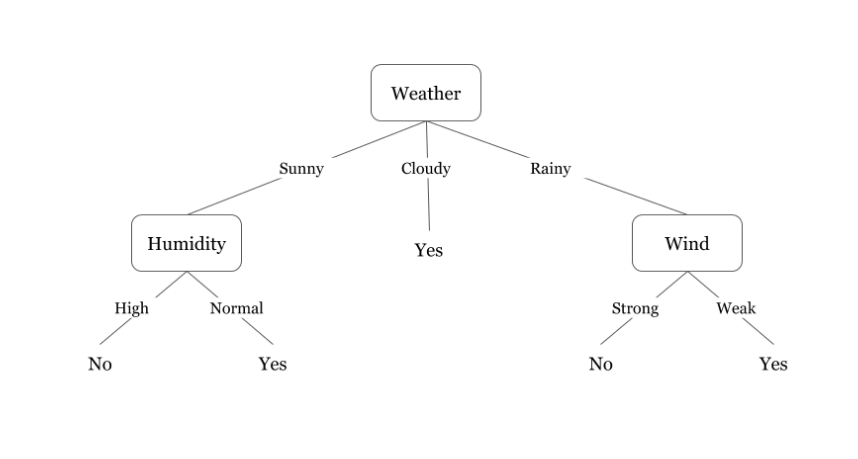
\includegraphics[scale=0.3]{decision-tree.png}
  \caption{Graphical representation of a decision tree on the problem: Should we play badminton or not based on weather conditions}
  \label{fig:decision-tree}
\end{figure}

As you can see, a tree is a collection of if-then conditional rules to reach a binary decision “yes-no” (we only illustrated  binary classification
for our purpose, but it can also classify labels) \cite{6}.

For our purpose, we are using decision trees in an ensemble, more accurately, a random forest, one of the most famous bagging methods, particularly famous for feature selection, a deciding factor in our decision to conduct experiments using this method.
This model works by spawning multiple decision trees each with a random subset of features and training data, it then pools the predictions together
and takes the average, take this as a multitude of humans making predictions about a specific matter, if the matter is hardly predictable, pooling and
averaging predictions can help reach a more precise result \cite{10}.
The prediction results using the Random Forest classifier with our current limited set of 9 features are demonstrated in tables
\autoref{fig:20-trees}, \autoref{fig:200-trees}, and \autoref{fig:500-trees} in the appendix.

As the results show in the tables, using the random forest method improves the accuracy to about 68\% which is the most promising result we have so far.
However, when looking at the variance and the training set accuracy, it shows us that the model is prone to overfitting, especially when the number of bagged trees reaches about 500, and the accuracy starts dropping.
For this reason, we decided in the following experiments, that a maximum depth for each considered decision tree should be set.


\subsection{Feature Post-processing: selecting the right features}
At this stage, lots of features have been extracted and utilised.
As elaborated in the data preprocessing section, both quality and quantity of the features play a vital role in the classification process.
Therefore, we decided to conduct feature post-processing  before adding more features.

\subsubsection{Imputation and Feature Importance}

In the conducted experiments, missing values are filled by dummy values or labels like ``missing'' or ``unknown''.
However, as discussed in the previous section, missing keywords should be replaced by the mode of each class, the real disaster class and the fake disaster ones.
Thus, a simple imputation by replacing those dummy fillers with corresponding mode values is implemented.
However, surprisingly, the prediction accuracy compared to before shows no noticeable improvement.
This is shown in \autoref{fig:replace-keyword-svc} in the appendix.

Additionally, we examine the feature importance by looking into the top-10 features that are selected by the random forest classifier.
In the appendix, \autoref{fig:top10-features-without-text} shows the top-10 features without text data and  \autoref{fig:important-features} illustrates the important features in the text data.
After analysis, each elected feature category plays an important role in the classification process.

\subsubsection{Polynomial Feature Extension}

Without using more NLP features, the simplest way to achieve massive features is to create new features based on existing features.
One of the approaches is to generate polynomial and interaction features the way resembles that of the polynomial kernel trick.
To this end, a polynomial feature generator from Scikit-learn library is inserted into the middle of the pipeline.

Originally, 38278 features including all text data have been used in previous experiments.
After inserting a polynomial order-two feature generator, the number of features of each data point is extended to 767869266 (about 770 million).
However, when feeding this amount of features into the random forest (our current best model) the training process could not be accomplished after 5
hours of training in the supercomputer DAS5 \cite{x5}, we thus decided to go with the SVC model with the rbf kernel.
The result is shown in table \autoref{fig:svc-rbf-kernel} in the appendix.

To our surprise, the performance did not improve as expected.
Therefore, we conclude that more features do help in terms of the classification only if the added features are relevant and carefully selected.

\subsection{Final Model Selection: Using full NLP feature set}
Finally, after several experiments, the ideal computational models that fit into our scenario are narrowed down to Random Forest.
At this final stage, we will make use of all NLP features described in \autoref{tab:feature-stats} together with the 5 entity-related features to evaluate the models.

\subsubsection{The Black-Box - Neural Net }
Before our final run of  the Random Forest model, it would be really interesting to see how all the features perform in a black-box neural network.
We thus chose the most straightforward NN method, Multi-layer Perceptron (MLP) classifier \cite{x6} to see whether there would be any promising results.
Again we provide a usability case study \cite{8} on why this model would be a promising choice. The results of this experiment are shown in \autoref{fig:mlp-all-features} and \autoref{fig:mlp-all-features-2000} in the appendix.

As illustrated in the resulting tables, there is indeed small performance gain by enlarging the neural  network.
However, considering the exponential increase of the training and evaluation time, we have to give up this method and stick with the Random Forest model.

\subsubsection{Tuning Hyperparameters of the final model - Random Forest}
Since examining the best number of trees and the maximum number considered for each tree are known to be the most time-consuming part, we, therefore,
make tuning of these two parameters a stand-alone process by drawing the out-of-bag (OOB) error curve \cite{x7} in order to see the convergence region so that we can to narrow down the range of the parameters and in turn shrink the random search grid.

\begin{figure}[h]
  \centering
  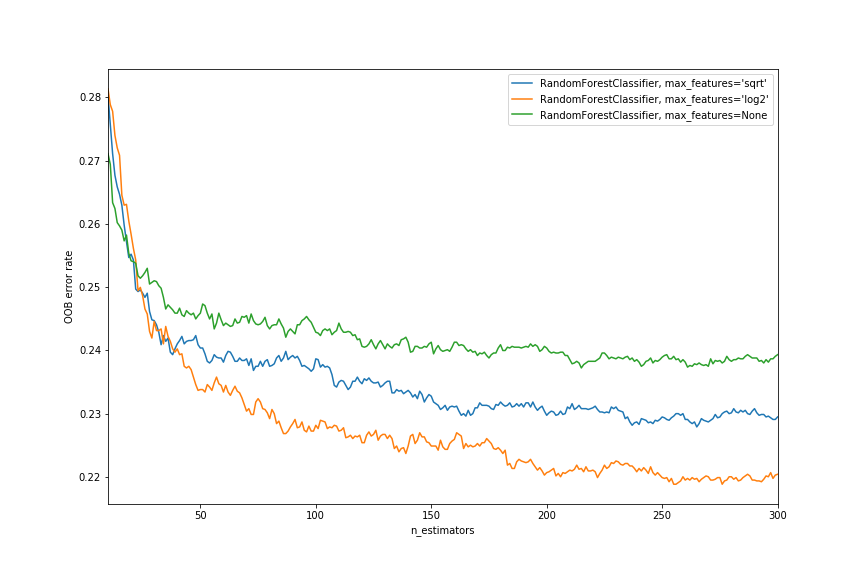
\includegraphics[scale=0.3]{curve.png}
  \caption{}
  \label{fig:curve}
\end{figure}


By setting up 3 pipelines with different \verb|max_features| parameters, we continually tune their \verb|n_estimators| parameters which resulted in
the OOB error curve showing in \autoref{fig:curve} in the appendix.

Based on the OOB error curve that we have, the best parameter for \verb|max_features| would be \verb|sqrt|.
For the \verb|n_estimation| parameter, there is a clear convergence around 250.
Thus, we finally shrink down the parameter distribution into the following,

\begin{verbatim}
random_distro ={
     'bootstrap': [True, False],
     'max_depth': [10, 20, 30, 40, 50, 60, 70, 80, 90, 100, None],
     'max_features': ['sqrt'],
     'min_samples_leaf': [1, 2, 4, 6, 8],
     'min_samples_split': [2, 5, 10],
     'n_estimators': [220, 250, 270]
}
\end{verbatim}


Further, a randomized search on hyperparameters is conducted using the Scikit-Learn library.
The result of the random search is shown in \autoref{fig:base-random} in the appendix.

\begin{verbatim}
{'n_estimators': 250,
 'min_samples_split': 6,
 'min_samples_leaf': 4,
 'max_features': 'sqrt',
 'max_depth': 80,
bootstrap': True}
\end{verbatim}

By comparing the base model of the random forest whose performance is shown in table \autoref{fig:random-hyper} in the appendix, an improvement on the cross-validation accuracy of about 3\% can be concluded and, perhaps most importantly, according to the training set accuracy, the tuned model less prone to be overfitting.

  \section{Results and evaluation}
\begin{figure}[h]
  \centering
  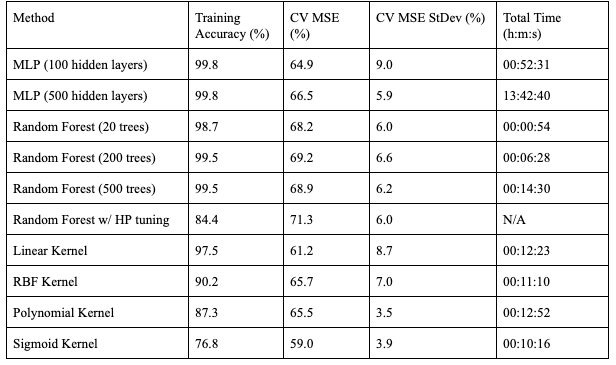
\includegraphics[scale=0.5]{results-table.png}
  \caption{}
  \label{fig:results-table}
\end{figure}

Table \autoref{fig:results-table} is a tabulated summary of the results from the models (as described in the experimental section) with the following; Accuracy of the model, Cross-Validation MSE and its standard deviation, the sum of the evaluation and training time and the section where this is discussed.

After evaluating all these models, we decided to explore the random forest further. Despite the NLP producing satisfactory results, the time to finish is prohibitive.

  \section{Conclusions}
In conclusion, linguistic features extracted from the NLP pipeline do improve the classification of disaster tweets when compared to classically derivable features.
We can conclude this because we extracted features from the text using an NLP pipeline, which yielded better results when compared to not doing so.
This result was observed because the NLP pipeline can extract structure from the text; this structure is embedded in the parts-of-speech that are in a tweet and the entities that are referred to.
 The NLP pipeline can also lemmatize words, which is useful for normalizing natural language for further processing.
This structure is then given to the models in a format that they can work with (vectors), which they can then work with to generate results.
Without these structures, the models are working with char arrays, which are ASCII values.
The baseline method (Linear SVC) yielded a result of 62\% prediction accuracy, and if you compare this to the accuracy after including NLP features, then an increase is observable.
This result is due to adding a small number of NLP-related features, but not all of them.
According to the test set accuracy, the first noticeable result was that we achieved the highest observed score after adding the NLP features.
Additionally, the test set accuracy is better than training accuracy because the overfitting issue did not occur due to the tuning of the hyperparameters (which limits the capacity of the tree model to overfit).

  \section{Discussion}
In this report, we demonstrate the results of various machine learning models in the task of natural language classification.
The end goal was to explore potential solutions to the problem of classifying tweets if they pertain to disasters or not.
With some success, we demonstrated that this is possible but not with high levels of confidence.
This lack of success stems from the problem statement being overly broad, in that it is not precisely clear what a disaster is and what is not.
There is not an authoritative source of truth that defines what is and is not a disaster because the meaning of this word is different according to different people.
Rightly so as different people have different perspectives and sets of values.
For example, to Donald Trump, the North American Free Trade Agreement is a disaster.
However, citizens of Mexico would say that it is an overwhelming success that has brought wealth and prosperity to their nation.
So is NAFTA a disaster or not? To Americans that worked in Automotive part suppliers (brakes, engines, etc.) NAFTA was a disaster since it decreased the number of available jobs in the country, but the opposite is true for Mexico and other trading partners of the US.
This begs the question, to whom would such an intelligent system serve? Americans? It could, but it would be unfair.
Therefore the scope of this problem needs to be narrowed down to something more specific that is unquestionably objective.
Without the problem adequately modeled, there is no set of equations that can consistently deliver accurate results for all cases.


One way to improve this system is to target, for example, natural disasters or automotive accidents.
An additional improvement would be to include a knowledge base that allows the system to understand that, for example, Kansas is situated in tornado valley, and so if a tweet becomes geotagged from Kansas, then it is more likely about a disaster.
This knowledge-base could also have a memory, that if there is a known disaster occurring in a geographical area, then tweets from that area will be much more likely to be about a disaster.


If this system were to be designed and implemented, then a thorough discussion about the acceptable level of risk associated with false positives and negatives.
As in how costly would a mistake be from this system trying to classify tweets? It is conceivable that if the risks are low, then it does not warrant a machine learning solution and all the complexity that comes from it.
Along this vein of discussion, perhaps no classifier is the best classifier.
Twitter could conceivably reserve a keyword in their service to flag to some trivial system that a particular tweet is, in fact, about a disaster.
If a user wants to let others know that they are in a disaster, then they can use it.
This system could be abused or misused, but the same holds for the machine learning models.


Regardless of the implementation, this system would be incredibly useful to organizations that dispatch critical resources to regions affected by disasters.
Such a system would allow for a more automated and proactive process that could make the difference in having a memorable disaster or a mundane event.


  \printbibliography

  \clearpage

\section{Appendix}
\begin{figure}[h!]
  \centering
  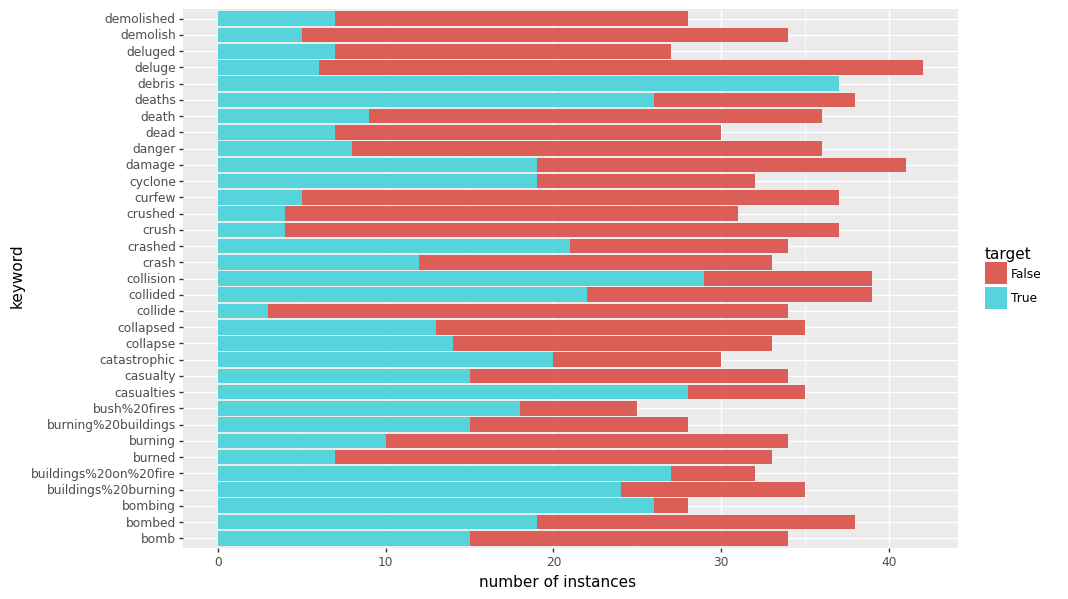
\includegraphics[scale=0.5]{keywords-vs-target.png}
  \caption{}
  \label{fig:keywords-vs-target}
\end{figure}

\begin{figure}[h!]
  \centering
  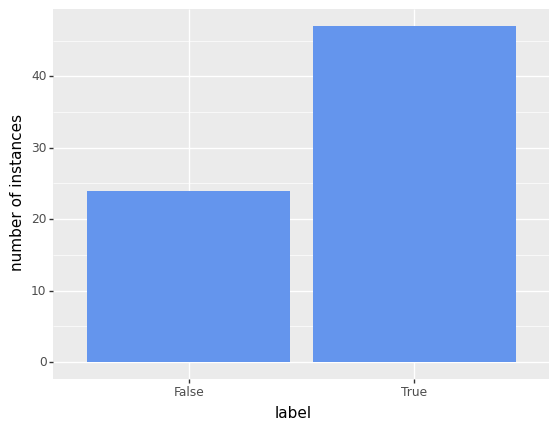
\includegraphics[scale=0.5]{mentioned-news.png}
  \caption{}
  \label{fig:mentioned-news}
\end{figure}

\begin{figure}[h!]
  \centering
  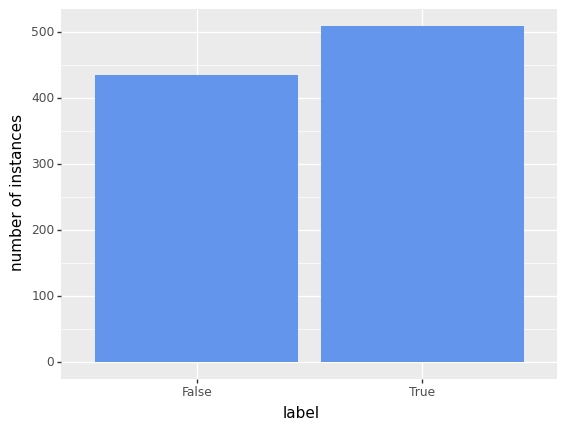
\includegraphics[scale=0.5]{contains-l1.png}
  \caption{}
  \label{fig:contains-l1}
\end{figure}

\begin{figure}[h!]
  \centering
  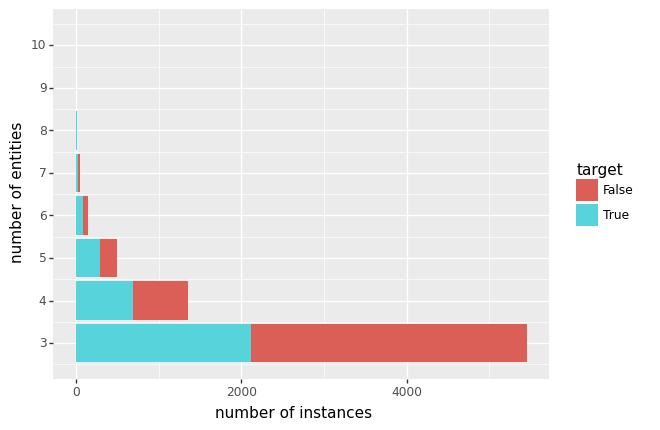
\includegraphics[scale=0.5]{num-ents-vs-target.png}
  \caption{}
  \label{fig:num-ents-vs-target}
\end{figure}


\begin{figure}[h!]
  \centering
  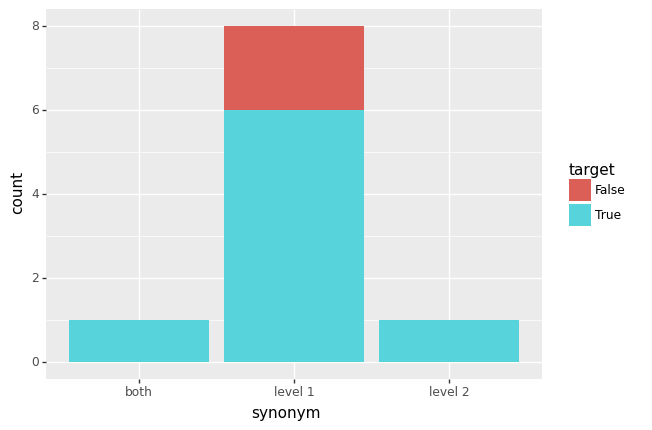
\includegraphics[scale=0.5]{hashtags-contain-synonyms.png}
  \caption{}
  \label{fig:hashtags-contain-synonyms}
\end{figure}

\begin{figure}[h!]
     \centering
     \begin{subfigure}[b]{0.42\textwidth}
         \centering
         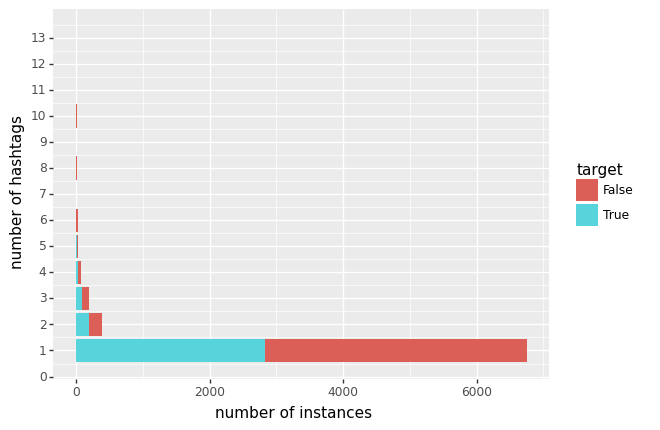
\includegraphics[width=\textwidth]{num-hashtags-vs-target.png}
         \caption{}
         \label{fig:num-hashtags-vs-target}
     \end{subfigure}
     \begin{subfigure}[b]{0.42\textwidth}
         \centering
         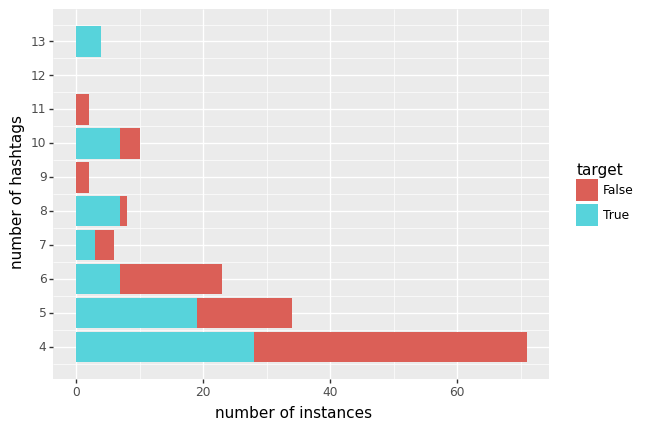
\includegraphics[width=\textwidth]{num-hashtags-vs-target-zoomed.png}
         \caption{}
         \label{fig:num-hashtags-vs-target-zoomed}
     \end{subfigure}
        \caption{}
        \label{fig:num-hashtags-graphs}
\end{figure}

\begin{figure}[h!]
     \centering
     \begin{subfigure}[b]{0.42\textwidth}
         \centering
         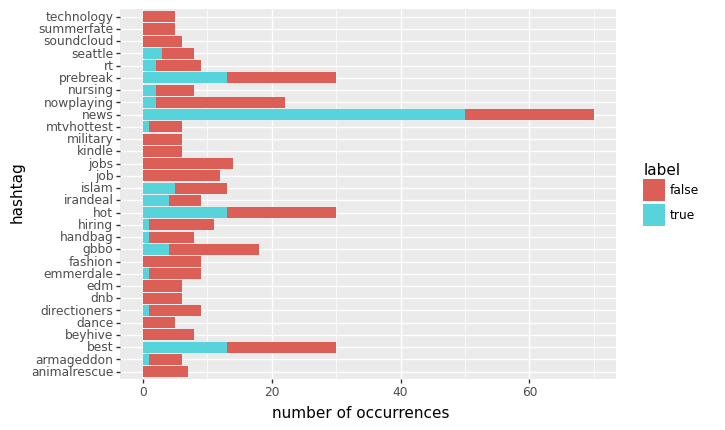
\includegraphics[width=\textwidth]{top-30-hashtags-false.png}
         \caption{}
         \label{fig:top-30-hashtags-false}
     \end{subfigure}
     \begin{subfigure}[b]{0.42\textwidth}
         \centering
         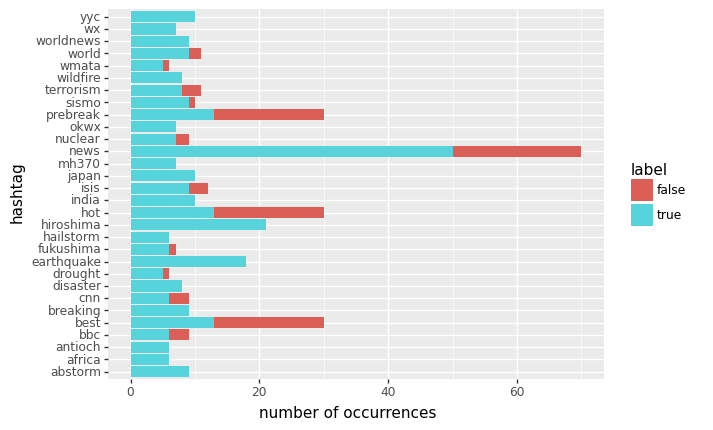
\includegraphics[width=\textwidth]{top-30-hashtags-true.png}
         \caption{}
         \label{fig:top-30-hashtags-true}
     \end{subfigure}
        \caption{}
        \label{fig:top-30-hashtags-graphs}
\end{figure}

\begin{table}[h]
  \centering
  \begin{tabular}{| l | p{0.4 \linewidth}|}
    \hline
    \textbf{Feature} & \textbf{Percentage of total instances with a value for the feature} \\ \hline
    Contains keyword & 100\% \\ \hline
    Contains location & 66.92\% \\ \hline
    Contains hashtag & 22.44\% \\ \hline
    Contains hashtag with level 1 synonym of "disaster" & 0.12\% \\ \hline
    Contains hashtag with level 2 synonym of "disaster" & 0.03\% \\ \hline
    Contains subject & 52.9\% \\ \hline
    Contains verb & 79.23\% \\ \hline
    Contains object & 79.39 \\ \hline
    Text contains level 1 synonym of "disaster" & 12.58\% \\ \hline
    Text contains level 2 synonym of "disaster" & 5.1\% \\ \hline
    Text contains words relating to damage  & 8.0\% \\ \hline
    News organisation mentioned & 0.95\% \\ \hline
    Relief organisation mentioned & 0.04\% \\ \hline
    Contains mentions & 25.4\% \\ \hline
    Contains one or more organisations & 59.72\% \\ \hline
    Contains one or more geopolitical entities & 15.19\% \\ \hline
    Contains one or more facilities & 1.73\% \\ \hline
  \end{tabular}
  \caption{}
  \label{tab:feature-stats}
\end{table}


\begin{figure}[h]
  \centering
  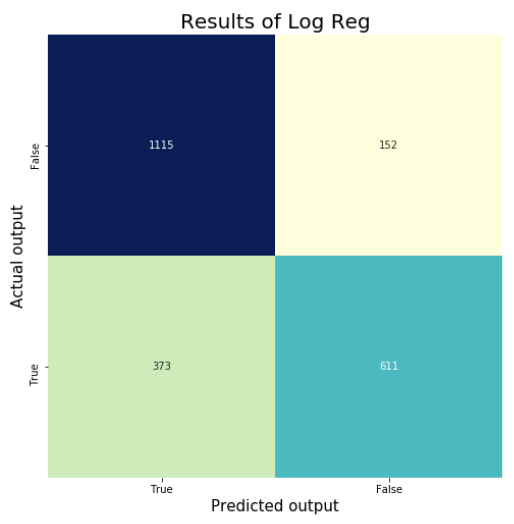
\includegraphics[scale=0.5]{confusion-matrix.png}
  \caption{Confusion matrix of 30\% of the tweets}
  \label{fig:confusion-matrix}
\end{figure}

\begin{figure}[h]
  \centering
  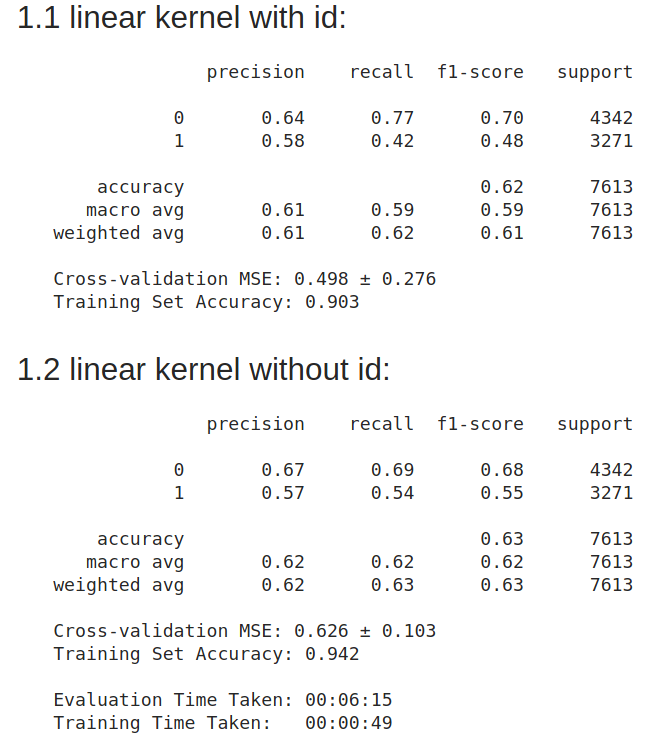
\includegraphics[scale=0.5]{feature-pre-elim-metrics.png}
  \caption{}
  \label{fig:feature-pre-elim-metrics}
\end{figure}

\begin{figure}[h]
  \centering
  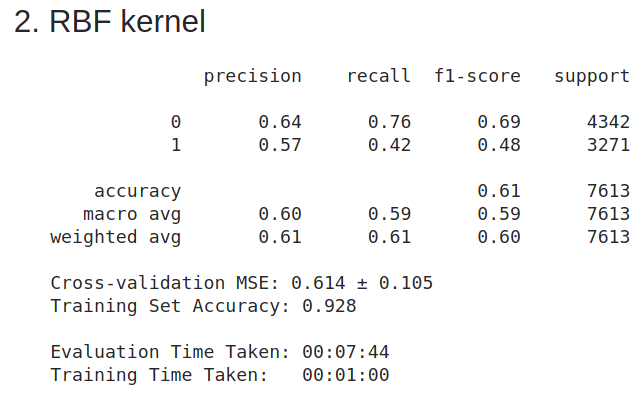
\includegraphics[scale=0.5]{rbf-kernel-tricks.png}
  \caption{}
  \label{fig:rbf-kernel-tricks}
\end{figure}

\begin{figure}[h]
  \centering
  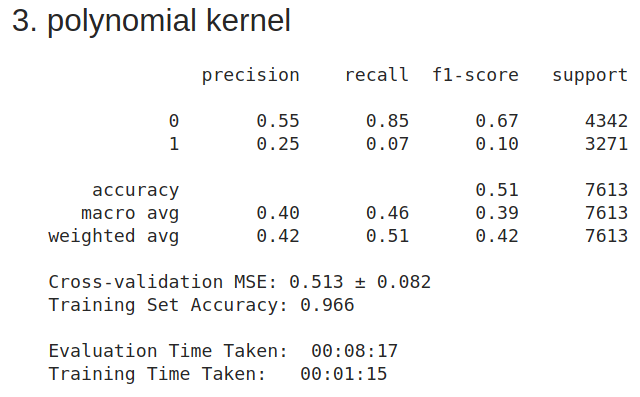
\includegraphics[scale=0.5]{poly-kernel-tricks.png}
  \caption{}
  \label{fig:poly-kernel-tricks}
\end{figure}

\begin{figure}[h]
  \centering
  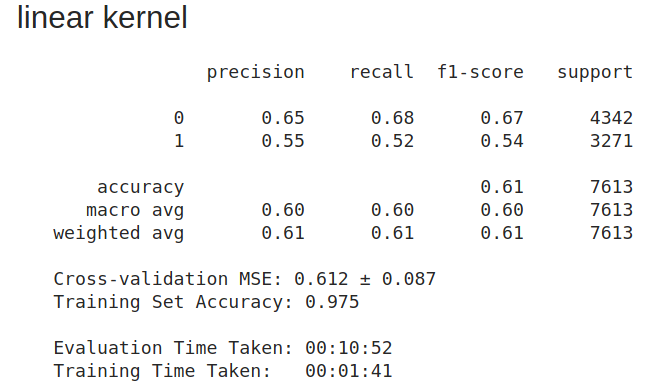
\includegraphics[scale=0.5]{linear-kernel-svc.png}
  \caption{}
  \label{fig:linear-kernel-svc}
\end{figure}

\begin{figure}[h]
  \centering
  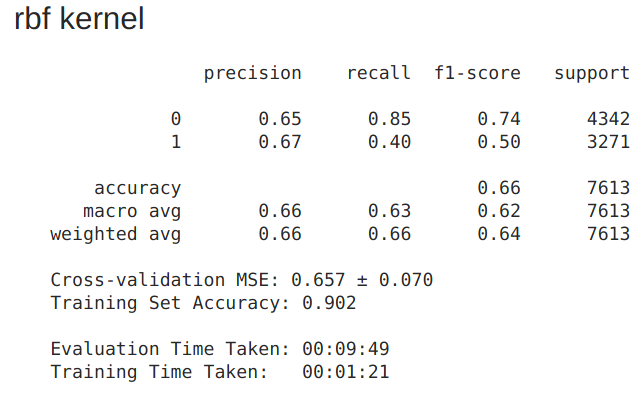
\includegraphics[scale=0.5]{rbf-kernel-svc.png}
  \caption{}
  \label{fig:rbf-kernel-svc}
\end{figure}

\begin{figure}[h]
  \centering
  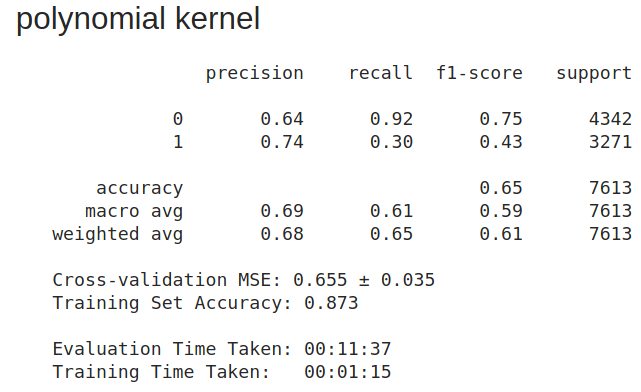
\includegraphics[scale=0.5]{poly-kernel-svc.png}
  \caption{}
  \label{fig:poly-kernel-svc}
\end{figure}

\begin{figure}[h]
  \centering
  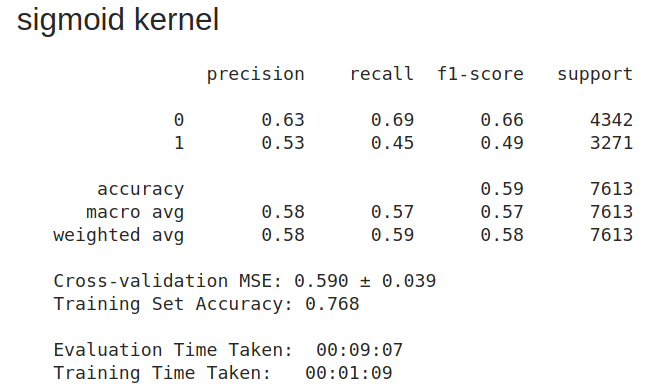
\includegraphics[scale=0.5]{sigmoid-kernel-svc.png}
  \caption{}
  \label{fig:sigmoid-kernel-svc}
\end{figure}

\begin{figure}[h]
  \centering
  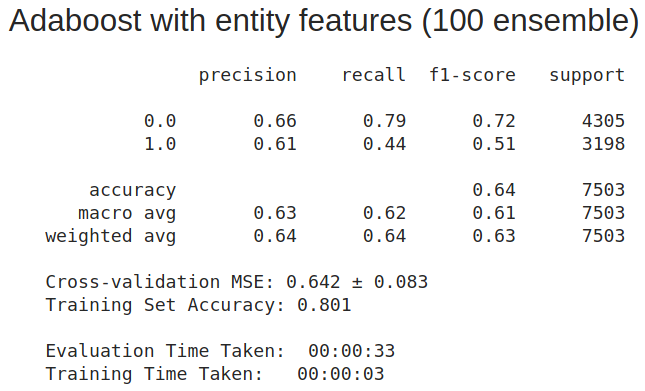
\includegraphics[scale=0.5]{adaboost.png}
  \caption{}
  \label{fig:adaboost}
\end{figure}

\begin{figure}[h]
  \centering
  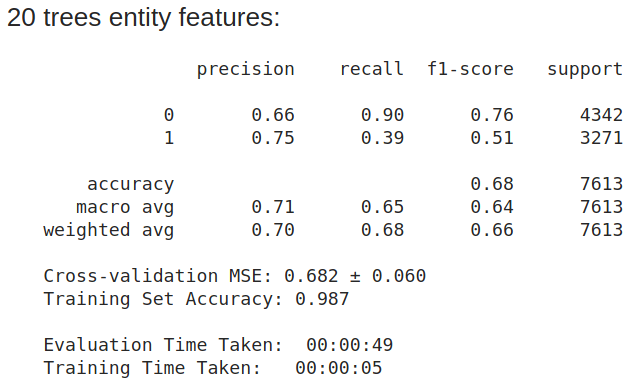
\includegraphics[scale=0.5]{20-trees.png}
  \caption{}
  \label{fig:20-trees}
\end{figure}

\begin{figure}[h]
  \centering
  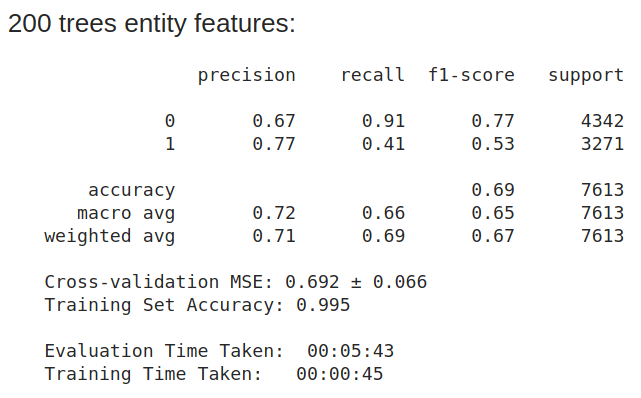
\includegraphics[scale=0.5]{200-trees.png}
  \caption{caption}
  \label{fig:200-trees}
\end{figure}

\begin{figure}[h]
  \centering
  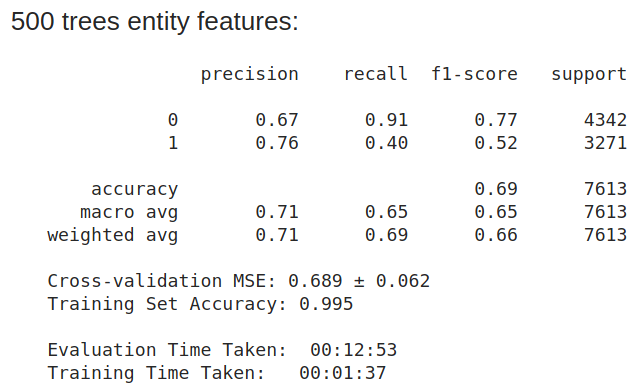
\includegraphics[scale=0.5]{500-trees.png}
  \caption{}
  \label{fig:500-trees}
\end{figure}

\begin{figure}[h]
  \centering
  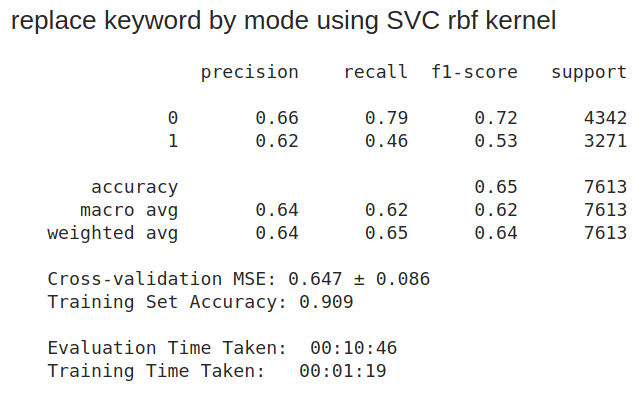
\includegraphics[scale=0.5]{replace-keyword-svc.png}
  \caption{}
  \label{fig:replace-keyword-svc}
\end{figure}

\begin{figure}[h]
  \centering
  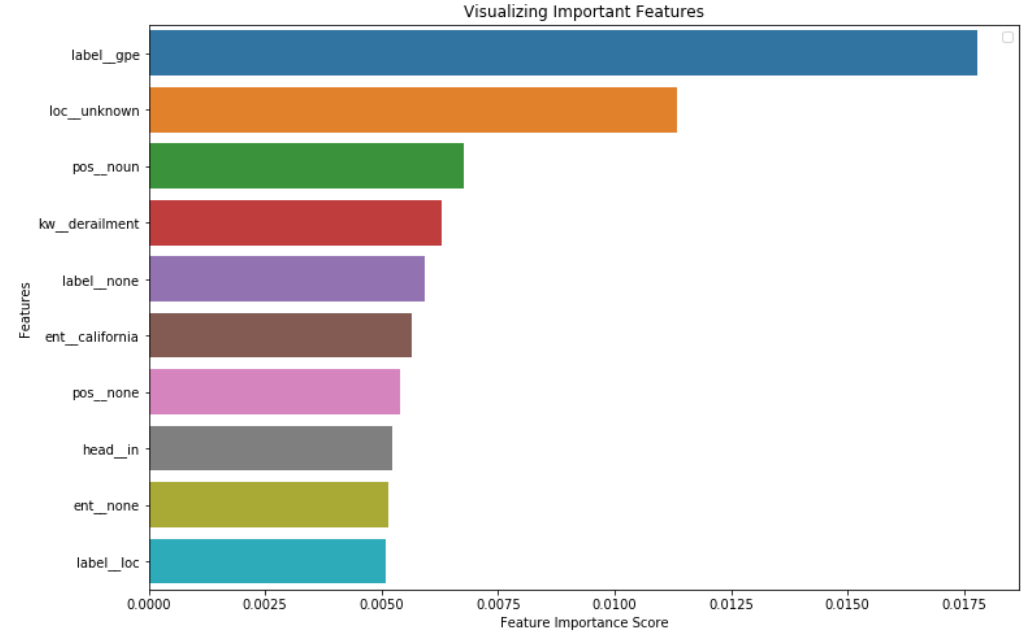
\includegraphics[scale=0.5]{top10-features-without-text.png}
  \caption{}
  \label{fig:top10-features-without-text}
\end{figure}

\begin{figure}[h]
  \centering
  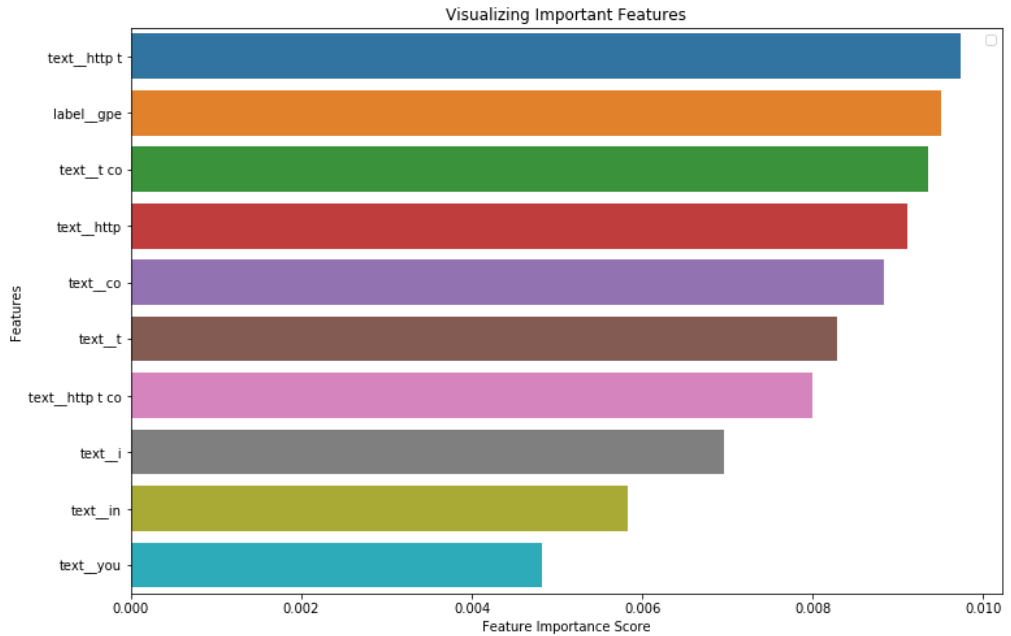
\includegraphics[scale=0.5]{important-features.png}
  \caption{}
  \label{fig:important-features}
\end{figure}

\begin{figure}[h]
  \centering
  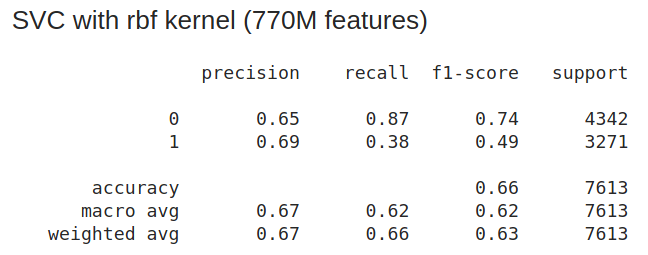
\includegraphics[scale=0.5]{svc-rbf-kernel.png}
  \caption{}
  \label{fig:svc-rbf-kernel}
\end{figure}

\begin{figure}[h]
  \centering
  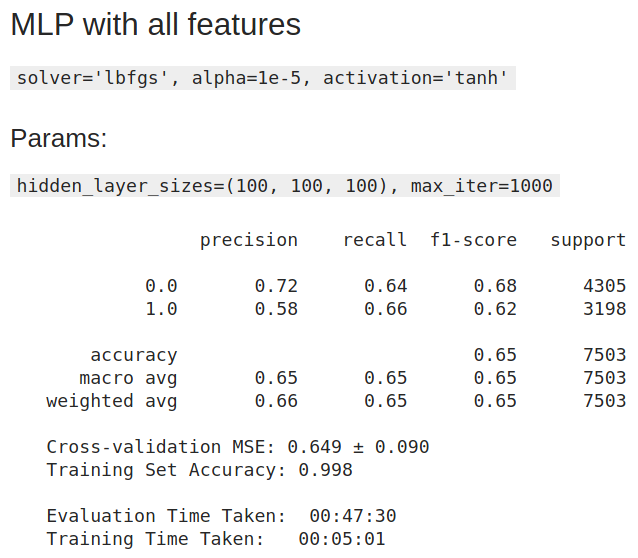
\includegraphics[scale=0.5]{mlp-all-features.png}
  \caption{}
  \label{fig:mlp-all-features}
\end{figure}

\begin{figure}[h]
  \centering
  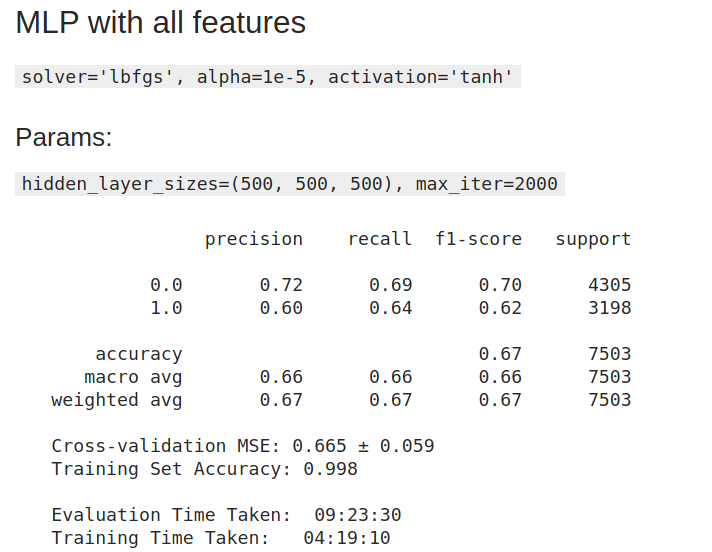
\includegraphics[scale=0.5]{mlp-all-features-2000.png}
  \caption{}
  \label{fig:mlp-all-features-2000}
\end{figure}

\begin{figure}[h]
  \centering
  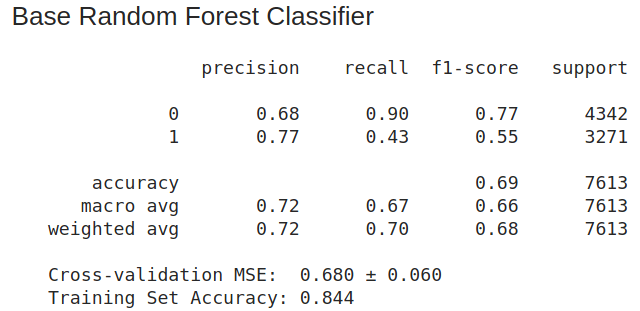
\includegraphics[scale=0.5]{base-random.png}
  \caption{}
  \label{fig:base-random}
\end{figure}

\begin{figure}[h]
  \centering
  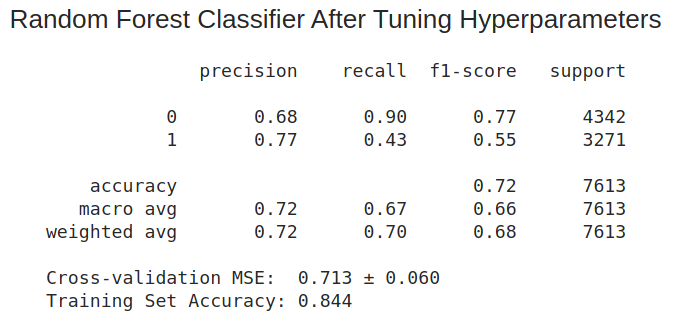
\includegraphics[scale=0.5]{random-hyper.png}
  \caption{}
  \label{fig:random-hyper}
\end{figure}

\end{document}
